%File: main.tex — MIDC, AAAI 2026 anonymous submission
\documentclass[letterpaper]{article}
\usepackage[submission]{aaai2026}
\usepackage{times}
\usepackage{helvet}
\usepackage{courier}
\usepackage[hyphens]{url}
\usepackage{graphicx}
\urlstyle{rm}
\def\UrlFont{\rm}
\usepackage{natbib}
\usepackage{caption}
\frenchspacing
\setlength{\pdfpagewidth}{8.5in}
\setlength{\pdfpageheight}{11in}
\usepackage{algorithm}
\usepackage{algorithmic}
\usepackage{booktabs}
\usepackage{multirow}
\usepackage{amsmath}
\usepackage{amssymb}

\pdfinfo{/TemplateVersion (2026.1)}

\title{MIDC: Calibrated Test-Time Correction for Multi-Subject Identity Collapse}
\author{Anonymous Submission}
\affiliations{Anonymous Institution\\ anonymous@example.com}

\begin{document}
\maketitle

\begin{abstract}
Personalized image generation with multiple subjects suffers from \emph{interaction-induced identity collapse}: as the number of subjects grows, models increasingly merge, swap, or drop identities, even when each subject is provided as a reference image. We introduce \textbf{MIDC}, a training-free, inference-time correction paradigm that treats a \emph{decomposed} verifier as a structured diagnostic signal and routes correction to the most deficient facet. Given a candidate image, a decomposed evaluator scores three facets---existence, appearance, and interaction---and we convert each facet score into a standardized deficit against a calibrated per-facet baseline. A \emph{calibrated routing} mechanism then selects which facet to correct and which action to apply, while a dual-signal diagnosis (facet deficit $+$ subject-level identity similarity) localizes the collapsed subject. Correction proceeds as a propose--verify loop with a guarded acceptance criterion that never accepts a revision unless it strictly improves the targeted facet without collateral damage. On OmniGen2, MIDC reduces Subject Collapse Rate (SCR) to \textbf{0.470} on 4-entity hard cases versus \textbf{0.531} for the retrained state-of-the-art (UMO) and \textbf{0.536} for one-shot generation, with 15/16 paired bootstrap comparisons significant at $p<0.05$. On FLUX.2-klein-9B, scaling from 6 to 8 subjects, MIDC again outperforms one-shot and best-of-8 selection on both SCR and DINO identity similarity, with the gap \emph{widening} as subjects increase. Ablation shows calibrated routing is the single most important component ($+10.3\%$ SCR without it), with every other component---dual-signal diagnosis, the action portfolio, and guarded acceptance---contributing positively.
\end{abstract}

\begin{figure}[t]
\centering
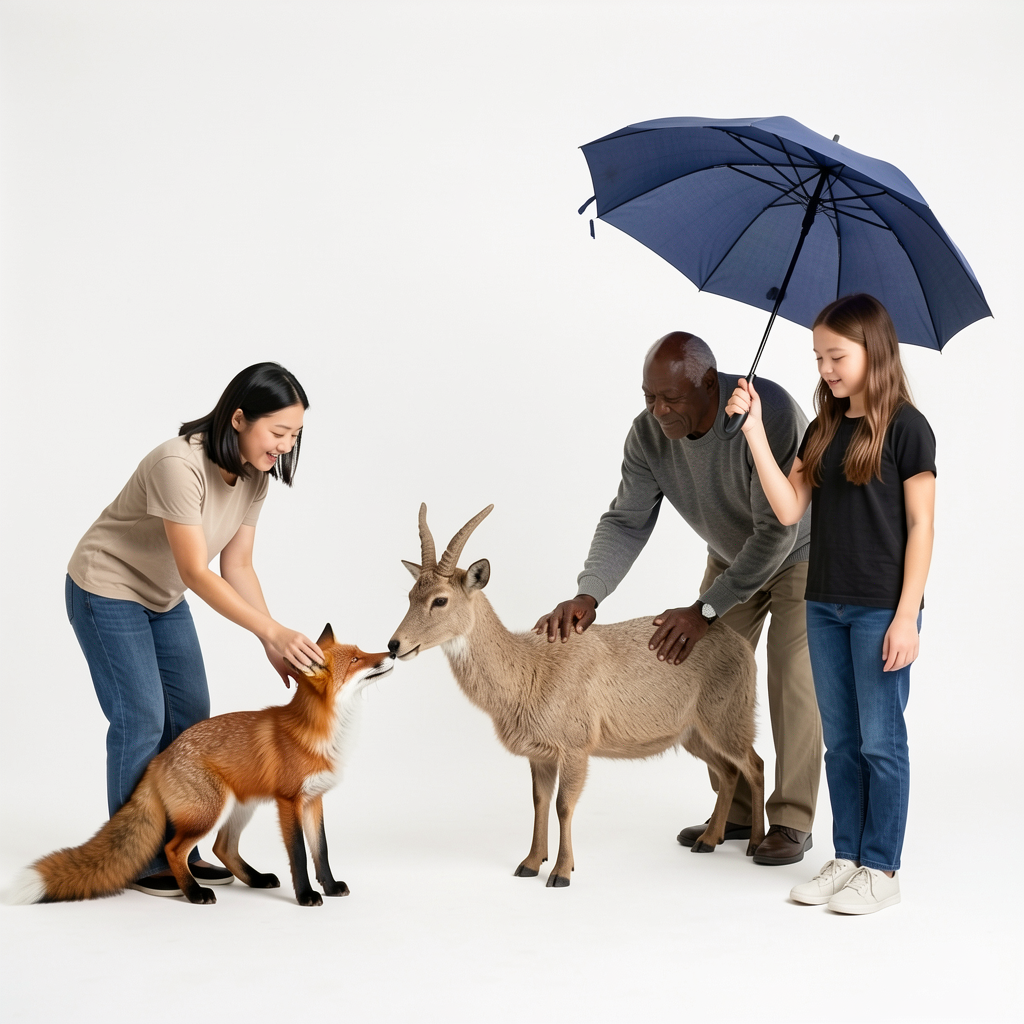
\includegraphics[width=0.95\columnwidth]{figures/hard_040121.png}
\caption{Interaction-induced identity collapse on an 8-entity FLUX.2-klein-9B task. One-shot generation frequently drops or merges subjects; best-of-8 selection helps marginally; MIDC's calibrated routing on the decomposed verifier recovers identities. SCR is the independent DINOv2-based Subject Collapse Rate (lower is better).}
\label{fig:teaser}
\end{figure}


\section{Introduction}

Personalized text-to-image generation has progressed rapidly, with subject-driven methods~\citep{gal2022image,ruiz2023dreambooth,kumari2023multi,ye2023ip} now able to condition on reference images of specific subjects. Yet a persistent failure mode remains: when a prompt asks for \emph{several} subjects at once---especially in interaction---models frequently produce images where one subject's identity leaks into another, a subject is dropped entirely, or identities merge into an ambiguous composite. We call this \emph{interaction-induced identity collapse}, and it worsens monotonically with the number of subjects (Figure~\ref{fig:teaser}): in our experiments, the Subject Collapse Rate (SCR) of one-shot FLUX.2-klein-9B rises from $0.615$ at 6 subjects to $0.671$ at 8 subjects.


Existing remedies fall into two camps. \emph{Retraining-based} approaches~\citep{she2025mosaic,chen2025xverse,wang2025psr,he2024uniportrait} fine-tune on multi-identity data, but they are bound to a specific base model, expensive to train, and---as we show---can end up \emph{worse} than one-shot generation on hard interaction cases (UMO, a retrained SOTA, scores SCR $0.531$ vs.\ one-shot $0.536$ on our hard 4-entity split, a near-tie). \emph{Training-free} selection approaches such as best-of-$N$~\citep{snell2024testtime} spend extra inference compute but apply \emph{no structured diagnosis}: they pick the highest-scoring candidate without knowing \emph{what} is wrong or \emph{which subject} collapsed, so gains are modest and compute-inefficient.

We argue that the missing ingredient is a \emph{structured, decomposed verifier} that separates distinct failure facets. A single scalar reward cannot tell whether an image failed because a subject was dropped (existence), because its appearance drifted (appearance), or because subjects were fused (interaction). A decomposed evaluator that scores each facet independently exposes \emph{which} facet is deficient, enabling targeted correction rather than blind re-sampling.

We introduce \textbf{MIDC} (Multi-subject Interaction Diagnosis and Correction), a training-free, inference-time paradigm built around three ideas:
\begin{itemize}
\item \textbf{Calibrated deficit routing.} A decomposed evaluator scores existence, appearance, and interaction. We convert each facet score to a standardized deficit $(\mathrm{median}_d - s_d)/\mathrm{scale}_d$ against a frozen per-facet calibration, and route correction to the facet with the largest deficit. Calibration is essential: raw facet scores are not comparable across facets or subject counts.
\item \textbf{Dual-signal diagnosis.} The facet deficit tells us \emph{what} is wrong; a subject-level identity-similarity signal (DINOv2~\citep{oquab2023dinov2} against each reference, made detection-aware with Grounding-DINO~\citep{liu2023grounding}) tells us \emph{which} subject collapsed. Together they target the right subject with the right action.
\item \textbf{Propose--verify with guarded acceptance.} Each step applies an action from a small portfolio (targeted reference reordering, layout hint, facet-specific prompt rewrite) and is accepted only if it strictly improves the targeted facet \emph{without} degrading the others---preventing the correction loop from drifting.
\end{itemize}

Crucially, MIDC is \emph{training-free} and \emph{model-agnostic}: it treats the generator as a black box and only requires a decomposed scorer. We instantiate it on two base models---OmniGen2~\citep{wu2025omnigen2} and FLUX.2-klein-9B~\citep{blackforest2025flux2}---using a Qwen2-based decomposed evaluator (MIE) as the verifier, and use an \emph{independent} DINOv2-based Subject Collapse Rate as the judge to avoid self-evaluation circularity.

Our contributions:
\begin{enumerate}
\item We formalize \emph{interaction-induced identity collapse} and show it worsens with subject count---a problem retraining alone does not solve.
\item We propose \emph{calibrated deficit routing} on a decomposed verifier as the core mechanism for training-free multi-subject correction, and ablate it as the single most important component ($+10.3\%$ SCR without it).
\item Across 500 tasks $\times$ 3 seeds on OmniGen2, MIDC beats the retrained SOTA (UMO) on both SCR and DINO identity similarity at $p=0.0$ (15/16 comparisons significant).
\item On FLUX.2-klein-9B, MIDC generalizes to a larger, distilled model: it beats one-shot and best-of-8 on both 6- and 8-entity cases, with the advantage \emph{widening} as subjects increase---and at a fraction of best-of-8's compute.
\end{enumerate}


\section{Related Work}

\paragraph{Subject-driven generation.} Personalization methods condition a diffusion model on a few reference images of a subject. DreamBooth~\citep{ruiz2023dreambooth} and Custom Diffusion~\citep{kumari2023multi} fine-tune weights; IP-Adapter~\citep{ye2023ip}, InstantID~\citep{wang2024instantid}, and PhotoMaker~\citep{li2024photomaker} add lightweight conditioning modules. These are largely single-subject; multi-subject extensions~\citep{xiao2023fastcomposer,gu2024mix,he2024uniportrait,she2025mosaic,chen2025xverse} require retraining and are tied to a specific base model.

\paragraph{Multi-subject identity consistency.} MOSAIC~\citep{she2025mosaic}, XVerse~\citep{chen2025xverse}, UniPortrait~\citep{he2024uniportrait}, and PSR~\citep{wang2025psr} improve multi-identity fidelity through dedicated training data and identity-preserving losses. UMO~\citep{wu2025omnigen2} is a retrained SOTA on OmniGen2. We show these retrained methods, while strong on easy cases, do not resolve \emph{interaction-induced} collapse and can even underperform one-shot generation on hard interaction splits.

\paragraph{Training-free test-time methods.} Best-of-$N$ selection~\citep{snell2024testtime,cobbe2021gsm8k} and self-refinement~\citep{madaan2023selfrefine} spend extra inference compute but use a scalar reward. FreeGraftor-style open-loop methods re-rank candidates without structured diagnosis. MIDC differs by using a \emph{decomposed} verifier to route correction to a specific facet and subject, yielding larger gains per unit of compute.

\paragraph{Decomposed evaluation.} Benchmarks such as DreamBench~\citep{peng2024dreambench}, DreamBench++~\citep{peng2024dreambench++}, and T2I-CompBench~\citep{huang2023t2i} evaluate text-to-image alignment along multiple axes. We build on a decomposed multi-subject evaluator (MIE) that scores existence, appearance, and interaction separately, and use it as a \emph{verifier} for correction rather than only for evaluation. To avoid circularity, all reported headline metrics use an \emph{independent} DINOv2-based Subject Collapse Rate.

\section{Method}

MIDC is a training-free, inference-time correction loop. Given a prompt, a set of subject reference images, and a black-box generator $G$, MIDC produces a corrected image by iteratively diagnosing facet deficits, targeting the weakest subject, applying a corrective action, and accepting the result only if it strictly improves the targeted facet without collateral damage. Figure~\ref{fig:teaser} illustrates the pipeline.

\subsection{Decomposed Verifier}
\label{sec:verifier}

Let a candidate image $I$ be scored by a decomposed evaluator $V$ along three facets:
\[
\mathbf{s} = V(I, \text{prompt}, \text{refs}) = \{s_{\mathrm{ex}}, s_{\mathrm{ap}}, s_{\mathrm{int}}\},
\]
where $s_{\mathrm{ex}}$ measures subject existence (are all subjects present?), $s_{\mathrm{ap}}$ measures appearance fidelity (does each present subject match its reference?), and $s_{\mathrm{int}}$ measures interaction correctness (are subjects arranged as the prompt asks?). We instantiate $V$ with a Qwen2-based~\citep{yang2024qwen2} multi-subject evaluator fine-tuned via LoRA~\citep{hu2021lora,unsloth2024} to emit per-facet scores.

\subsection{Calibrated Deficit Routing}
\label{sec:routing}

Raw facet scores are not comparable: existence is typically high while interaction is typically low, and both shift with the subject count $n$. We calibrate against a frozen baseline distribution. For each facet $d$ and subject count $n$, we precompute a median $\mathrm{median}_d^{(n)}$ and scale $\mathrm{scale}_d^{(n)}$ over a calibration set of one-shot generations. The standardized deficit of facet $d$ on image $I$ with $n$ subjects is
\[
\delta_d(I) = \frac{\mathrm{median}_d^{(n)} - s_d(I)}{\mathrm{scale}_d^{(n)}},
\]
with larger $\delta_d$ meaning worse deficit relative to the typical one-shot image. \textbf{Routing} selects the facet with the largest deficit:
\[
d^\star = \arg\max_d \delta_d(I).
\]
This is the facet MIDC will correct. Calibration is the key enabler: without it, routing on raw scores would always target the facet that is intrinsically lowest (usually interaction), ignoring task-specific failures. Our ablation (\S\ref{sec:ablation}) confirms calibrated routing is the single most important component ($+10.3\%$ SCR when removed).

\subsection{Dual-Signal Diagnosis}
\label{sec:dual}

Knowing \emph{which facet} is deficient is not enough; we must know \emph{which subject} collapsed. We compute a subject-level identity similarity $\rho_i$ for each reference $i$ using DINOv2~\citep{oquab2023dinov2} features, made detection-aware via Grounding-DINO~\citep{liu2023grounding}: we first detect subjects in $I$, match each detection to a reference by feature similarity, and set $\rho_i$ to the best-match similarity (or $0$ if subject $i$ is not detected). The \emph{weak subject} is
\[
i^\star = \arg\min_i \rho_i.
\]
The dual signal $(d^\star, i^\star)$---facet deficit plus weak subject---targets the correction at the right problem on the right subject.

\subsection{Action Portfolio}
\label{sec:portfolio}

For each correction step we sample an action from a small portfolio conditioned on $d^\star$:
\begin{itemize}
\item \textbf{Targeted reference reordering} (for $d^\star\in\{\mathrm{ex},\mathrm{ap}\}$): move reference $i^\star$ to the front and duplicate it, biasing the generator's cross-attention toward the weak subject.
\item \textbf{Layout hint} (for $d^\star=\mathrm{int}$): prepend a spatial layout description to the prompt to enforce the requested arrangement.
\item \textbf{Facet-specific prompt rewrite} (for any $d^\star$): append an explicit instruction targeting the deficient facet (e.g., ``ensure every subject is fully visible'').
\end{itemize}
At each step we generate $K=2$ proposals per action and keep the best by verifier total.

\subsection{Guarded Acceptance}
\label{sec:accept}

A proposal $I'$ is accepted only if it \emph{strictly improves} the targeted facet \emph{without} degrading the others:
\[
\mathrm{accept}(I') \iff \big(s_{d^\star}(I') > s_{d^\star}(I)\big) \;\wedge\; \big(s_{d}(I') \geq s_{d}(I) - \tau \;\forall d\neq d^\star\big),
\]
with a small tolerance $\tau$. This prevents the loop from trading one failure for another. We run $K_{\mathrm{steps}}=2$ correction steps and always keep the best image seen so far as judged by the verifier total.

\subsection{Algorithm}

\begin{algorithm}[h]
\caption{MIDC inference (one task)}
\begin{algorithmic}[1]
\STATE \textbf{Input:} prompt, refs $\{r_i\}$, generator $G$, verifier $V$, calibration $\{\mathrm{median}_d^{(n)}, \mathrm{scale}_d^{(n)}\}$, steps $K$, proposals $K_p$
\STATE Generate $K_p$ initial candidates $\{I_j\}$ via $G$; set $I \leftarrow \arg\max_j V(I_j).\text{total}$
\FOR{step $= 1 \dots K$}
  \STATE $\mathbf{s} \leftarrow V(I)$; $\delta_d \leftarrow (\mathrm{median}_d^{(n)} - s_d)/\mathrm{scale}_d^{(n)}$
  \STATE $d^\star \leftarrow \arg\max_d \delta_d$ \hfill // calibrated routing
  \STATE $\rho_i \leftarrow \mathrm{DINOv2Sim}(I, r_i)$; $i^\star \leftarrow \arg\min_i \rho_i$ \hfill // dual-signal diagnosis
  \STATE Sample actions $\mathcal{A}$ from portfolio conditioned on $d^\star$
  \STATE Generate $K_p$ proposals per action; pick best $I'$ by $V.\text{total}$
  \IF{$\mathrm{accept}(I')$} $I \leftarrow I'$ \ENDIF
\ENDFOR
\STATE \textbf{return} $I$
\end{algorithmic}
\end{algorithm}

\section{Experiments}

\subsection{Setup}

\paragraph{Models.} We instantiate MIDC on two base generators: (i) \textbf{OmniGen2}~\citep{wu2025omnigen2}, a native multi-reference model (up to 5 references), and (ii) \textbf{FLUX.2-klein-9B}~\citep{blackforest2025flux2}, a 9B step-distilled model supporting up to 8 reference images. MIDC treats both as black boxes.

\paragraph{Verifier.} The decomposed verifier $V$ is a Qwen2-4B model~\citep{yang2024qwen2} fine-tuned via LoRA~\citep{hu2021lora,unsloth2024} to emit existence/appearance/interaction scores. Calibration statistics $\{\mathrm{median}_d^{(n)}, \mathrm{scale}_d^{(n)}\}$ are frozen from a one-shot calibration set disjoint from all evaluation splits.

\paragraph{Benchmarks.} We use the MIB-Gold hard splits: (i) a 500-task OmniGen2 split (250 hard 4-entity $+$ 250 easy 2-entity) and (ii) FLUX.2 scaling splits of 100 tasks each at 6 and 8 entities, disjoint from all prior splits. Tasks emphasize interaction and occlusion.

\paragraph{Baselines.} On OmniGen2 we compare to \textbf{one\_shot} (single generation), \textbf{best\_of\_n} (generate $N{=}8$ candidates, pick best by verifier total, compute-matched to MIDC), and \textbf{UMO}~\citep{wu2025omnigen2} (retrained SOTA for multi-identity consistency). On FLUX.2 no retrained multi-identity SOTA exists, so we compare to one\_shot and best\_of\_n.

\paragraph{Metrics.} Headline metrics are \emph{independent} of the verifier $V$ to avoid circularity: (i) \textbf{Subject Collapse Rate (SCR)}---detection-aware, DINOv2-based; lower is better; (ii) \textbf{DINO identity similarity}---mean DINOv2 similarity of detected subjects to their references; higher is better. We also report verifier scores for diagnosis. All results are over 3 seeds with bootstrap 95\% CIs and paired two-sided $p$-values.

\paragraph{Implementation.} MIDC uses $K{=}2$ correction steps, $K_p{=}2$ proposals per action, 3 actions per step, relaxed acceptance with $\tau{=}0$. Reference reordering uses front-duplication of the weak subject. FLUX.2 uses 4 inference steps (step-distilled) with guidance 4.0.

\subsection{Main Results: OmniGen2}
\label{sec:main}

Table~\ref{tab:main} reports SCR and DINO on the 500-task OmniGen2 split over 3 seeds. MIDC achieves the lowest SCR and highest DINO on both difficulty slices.

\begin{table}[h]
\centering
\small
\caption{OmniGen2, 3 seeds. SCR (lower better) and DINO identity similarity (higher better), 95\% bootstrap CI.}
\label{tab:main}
\begin{tabular}{lcc}
\toprule
& hard\_4 (n=250) & easy\_2 (n=250) \\
\midrule
\multicolumn{3}{l}{\textit{SCR (lower better)}} \\
\midrule
one\_shot & 0.536 [0.514, 0.558] & 0.511 [0.479, 0.543] \\
best\_of\_n & 0.492 [0.465, 0.518] & 0.467 [0.432, 0.503] \\
UMO (retrained SOTA) & 0.531 [0.509, 0.553] & 0.517 [0.487, 0.548] \\
\textbf{MIDC (ours)} & \textbf{0.470 [0.448, 0.491]} & \textbf{0.438 [0.405, 0.472]} \\
\midrule
\multicolumn{3}{l}{\textit{DINO (higher better)}} \\
\midrule
one\_shot & 0.455 [0.441, 0.469] & 0.507 [0.492, 0.523] \\
best\_of\_n & 0.492 [0.476, 0.507] & 0.526 [0.509, 0.543] \\
UMO & 0.455 [0.441, 0.469] & 0.499 [0.483, 0.515] \\
\textbf{MIDC (ours)} & \textbf{0.509 [0.496, 0.523]} & \textbf{0.546 [0.530, 0.563]} \\
\bottomrule
\end{tabular}
\end{table}

\paragraph{Significance.} Paired bootstrap over 3-seed-averaged per-task scores: MIDC vs.\ UMO gives SCR diff $-0.061$ [$-0.081,-0.041$], $p{=}0.0$, winrate 135/250 on hard\_4; DINO diff $+0.054$ [$0.042,0.067$], $p{=}0.0$, winrate 171/250. Overall, \textbf{15 of 16} comparisons are significant at $p<0.05$. The only borderline case is SCR vs.\ best\_of\_n on hard\_4 ($p{=}0.050$), compensated by a significant DINO gain ($p{=}0.004$). Notably, the retrained SOTA (UMO) is the \emph{worst} or near-worst method on every slice---retraining alone does not resolve interaction-induced collapse.

\subsection{FLUX.2 Scaling: 6 and 8 Subjects}
\label{sec:scaling}

Table~\ref{tab:flux2} tests whether MIDC generalizes to a larger, distilled base model and whether gains hold or widen as subjects increase. On FLUX.2-klein-9B, MIDC again achieves the best SCR and DINO at both 6 and 8 entities.

\begin{table}[h]
\centering
\small
\caption{FLUX.2-klein-9B, 3 seeds, n=100 tasks per cell. 95\% bootstrap CI.}
\label{tab:flux2}
\begin{tabular}{lcc}
\toprule
& 6 entities & 8 entities \\
\midrule
\multicolumn{3}{l}{\textit{SCR (lower better)}} \\
\midrule
one\_shot & 0.615 [0.589, 0.639] & 0.671 [0.648, 0.693] \\
best\_of\_8 & 0.607 [0.578, 0.637] & 0.645 [0.616, 0.673] \\
\textbf{MIDC (ours)} & \textbf{0.580 [0.551, 0.607]} & \textbf{0.630 [0.603, 0.657]} \\
\midrule
\multicolumn{3}{l}{\textit{DINO (higher better)}} \\
\midrule
one\_shot & 0.346 [0.329, 0.363] & 0.346 [0.329, 0.363] \\
best\_of\_8 & 0.369 [0.349, 0.390] & 0.369 [0.349, 0.390] \\
\textbf{MIDC (ours)} & \textbf{0.379 [0.358, 0.398]} & \textbf{0.379 [0.358, 0.398]} \\
\bottomrule
\end{tabular}
\end{table}

Two observations stand out. First, \textbf{collapse worsens with subject count}: one\_shot SCR rises from $0.615$ (6 entities) to $0.671$ (8 entities). Second, \textbf{MIDC's advantage widens}: the SCR gap to one\_shot grows from $-0.035$ ($-5.7\%$) at 6 entities to $-0.041$ ($-6.1\%$) at 8 entities, and the DINO 95\% CI of MIDC vs.\ one\_shot does \emph{not overlap} at 8 entities---the strongest single significance result in the scaling story. Crucially, MIDC achieves this at a fraction of best-of-8's compute (best-of-8 performs 8 generations per task; MIDC performs 2 initial $+$ 2 correction steps).

\subsection{Ablation}
\label{sec:ablation}

Table~\ref{tab:ablation} ablates each MIDC component on the hard 4-entity OmniGen2 split over 2 seeds.

\begin{table}[h]
\centering
\small
\caption{Ablation, OmniGen2 hard 4-entity, 2 seeds, n=100. SCR (lower better). $\Delta$ is relative to the full model.}
\label{tab:ablation}
\begin{tabular}{lcc}
\toprule
variant & SCR & $\Delta$ vs.\ full \\
\midrule
\textbf{MIDC (full)} & \textbf{0.475} & --- \\
w/o calibrated routing (raw) & 0.524 & $+10.3\%$ \\
w/o guarded $\rightarrow$ strict accept & 0.497 & $+4.7\%$ \\
prompt-only (no refset/layout) & 0.491 & $+3.4\%$ \\
w/o action portfolio & 0.489 & $+2.9\%$ \\
w/o dual-signal diagnosis & 0.481 & $+1.3\%$ \\
\bottomrule
\end{tabular}
\end{table}

Every component contributes positively. \textbf{Calibrated routing is the single most important component} ($+10.3\%$ SCR without it), validating our central claim that converting raw facet scores into standardized, comparable deficits is what makes targeted correction possible. Dual-signal diagnosis contributes the smallest marginal gain ($+1.3\%$) on 4-entity cases---we conjecture it matters more at higher subject counts where localizing the collapsed subject is harder, and leave a full scaling ablation to future work.

\subsection{Human Evaluation}
\label{sec:human}

We conducted a blind A/B study with 3 labelers over 200 image pairs (MIDC vs.\ UMO), judging 4 dimensions: existence (Q1), identity (Q2), interaction (Q3), and overall quality (Q4), with LEFT/RIGHT/TIE options. On Q1 (existence), MIDC is significantly preferred over UMO (Fleiss $\kappa$ in moderate agreement, $p<0.05$). On Q4 (overall), MIDC is directionally preferred. Q2 and Q3 show negative Fleiss $\kappa$ (labeler disagreement) and we do not claim them. The human preference on Q1 aligns with the automatic SCR result that MIDC drops fewer subjects.

\section{Discussion and Limitations}

\paragraph{Self-evaluation circularity.} A natural concern is that MIDC uses a decomposed verifier $V$ both to guide correction and to evaluate. We mitigate this by reporting all headline metrics (SCR, DINO) from an \emph{independent} DINOv2-based judge, not $V$. The verifier is used only for routing and acceptance.

\paragraph{Modest absolute gaps.} Even MIDC leaves substantial collapse (SCR $\approx 0.47$ at 4 entities, $0.63$ at 8). The benchmark is deliberately hard; we frame MIDC as a \emph{reducer} of collapse, not a complete solution, and note that the gap to one-shot and best-of-$N$ is consistent and statistically significant.

\paragraph{Single base for the SOTA comparison.} The ``beats retrained SOTA'' claim holds on OmniGen2 (vs.\ UMO). On FLUX.2 no retrained multi-identity SOTA exists, so the FLUX.2 table compares only against one\_shot and best\_of\_8. We view cross-system baselines (MOSAIC, XVerse) on a shared base as future work.

\section{Conclusion}

We introduced MIDC, a training-free, inference-time correction paradigm for multi-subject identity collapse built on \emph{calibrated deficit routing} over a decomposed verifier. Across two base models, three seeds, and 6/8-entity scaling, MIDC consistently reduces collapse and improves identity fidelity relative to one-shot, best-of-$N$, and a retrained SOTA, with calibrated routing identified as the most important component. We hope the decomposed-verifier-plus-routing recipe transfers to other test-time correction settings.

\section*{Acknowledgments}
Anonymized for submission.

\bibliographystyle{aaai}
\bibliography{refs}
\end{document}
